\newpage
\section{Билет 16. Архитектуры информационных систем: "монолитная", клиент-серверная, многоуровневая. Одноранговые системы (peer-to-peer).}

\noindent {\large Компоненты архитектуры распределённой системы:}
\begin{enumerate}
\item \textit{Физическое оборудование и сеть}

Приложение запускается на компьютере определённого производителя, определённого типа памяти и т.д.

\item \textit{Операционная система.}

Устанавливается на физическое оборудование. Одна из задач операционной системы это предоставить единый интерфейс представления оборудования. То есть операционная система скрывает особенности оборудования. Например если написать программу на линукс, то она будет работать на любом линуксе, а также в нём есть принцип "всё есть файл", то есть и любой объект оборудования имеет интерфейс файла в этой системе. 

\item \textit{Промежуточное ПО (Middleware).}

Поверх операционной системы может работать программное обеспечение промежуточного слоя - Middleware.
Его задача - сокрытие неоднородности и предоставление базовых функций приложениям (удалённый вызов функции, примитивы передачи сообщений, многоадресная передача и т.п.).
То есть это набор сервисов, служб, функций которые полезны многим приложениям.

\item \textit{Приложения и сервисы.}

Непосредственно разработанное приложение.
\end{enumerate}

\noindent Цель каждого уровня - максимально скрыть сложность уровня, который был выше.\\
\\
{\large Различные системные архитектуры:}
\begin{enumerate}
\item \textbf{ Монолитное решение}

Всё работает на одном компьютере.

\textit{ Примечание: это не распределённая система.}

\item \textbf{ Клиент-серверная}

Поскольку базы данных как правило используется для совместной работы нескольких пользователей, она обычно вынесена на отдельный сервер. 
То есть существует программа клиент и программа сервер, а также какой-то протокол их общения, желательно открытый.

Базы данных различных разработчиков практически всегда отличаются, и взаимозаменяемости (открытости) на уровне протоколов почти всегда нет, поэтому она достигается за счёт стандартизации запросов (SQL).

\item \textbf{ Клиент-серверная с посредниками (proxy-сервер)}

Есть промежуточные сервера, которые со стороны клиента выглядят так же, как основной, но такой сервер ничего не делает, а просто перенаправляет запросы.\\
Иногда proxy-сервер может оптимизировать доступ к каналам связи, а именно закэшировать какие-то данные, которые часто запрашиваются.\\
Или же на proxy-сервере можно решать какие-то вопросы безопасности, например запрет прямого доступа к главному серверу, можно заходить только через proxy-сервер на котором происходит проверка политики безопасности.

\item \textbf{ Многоуровневая}
Может быть двух типов:
\begin{itemize}
\item
Многосерверная - сервис предоставляется совокупностью вычислительных процессов. Например репликация, которая реализована в виде нескольких общающихся процессов, но для клиента выглядят одним.\\
\\
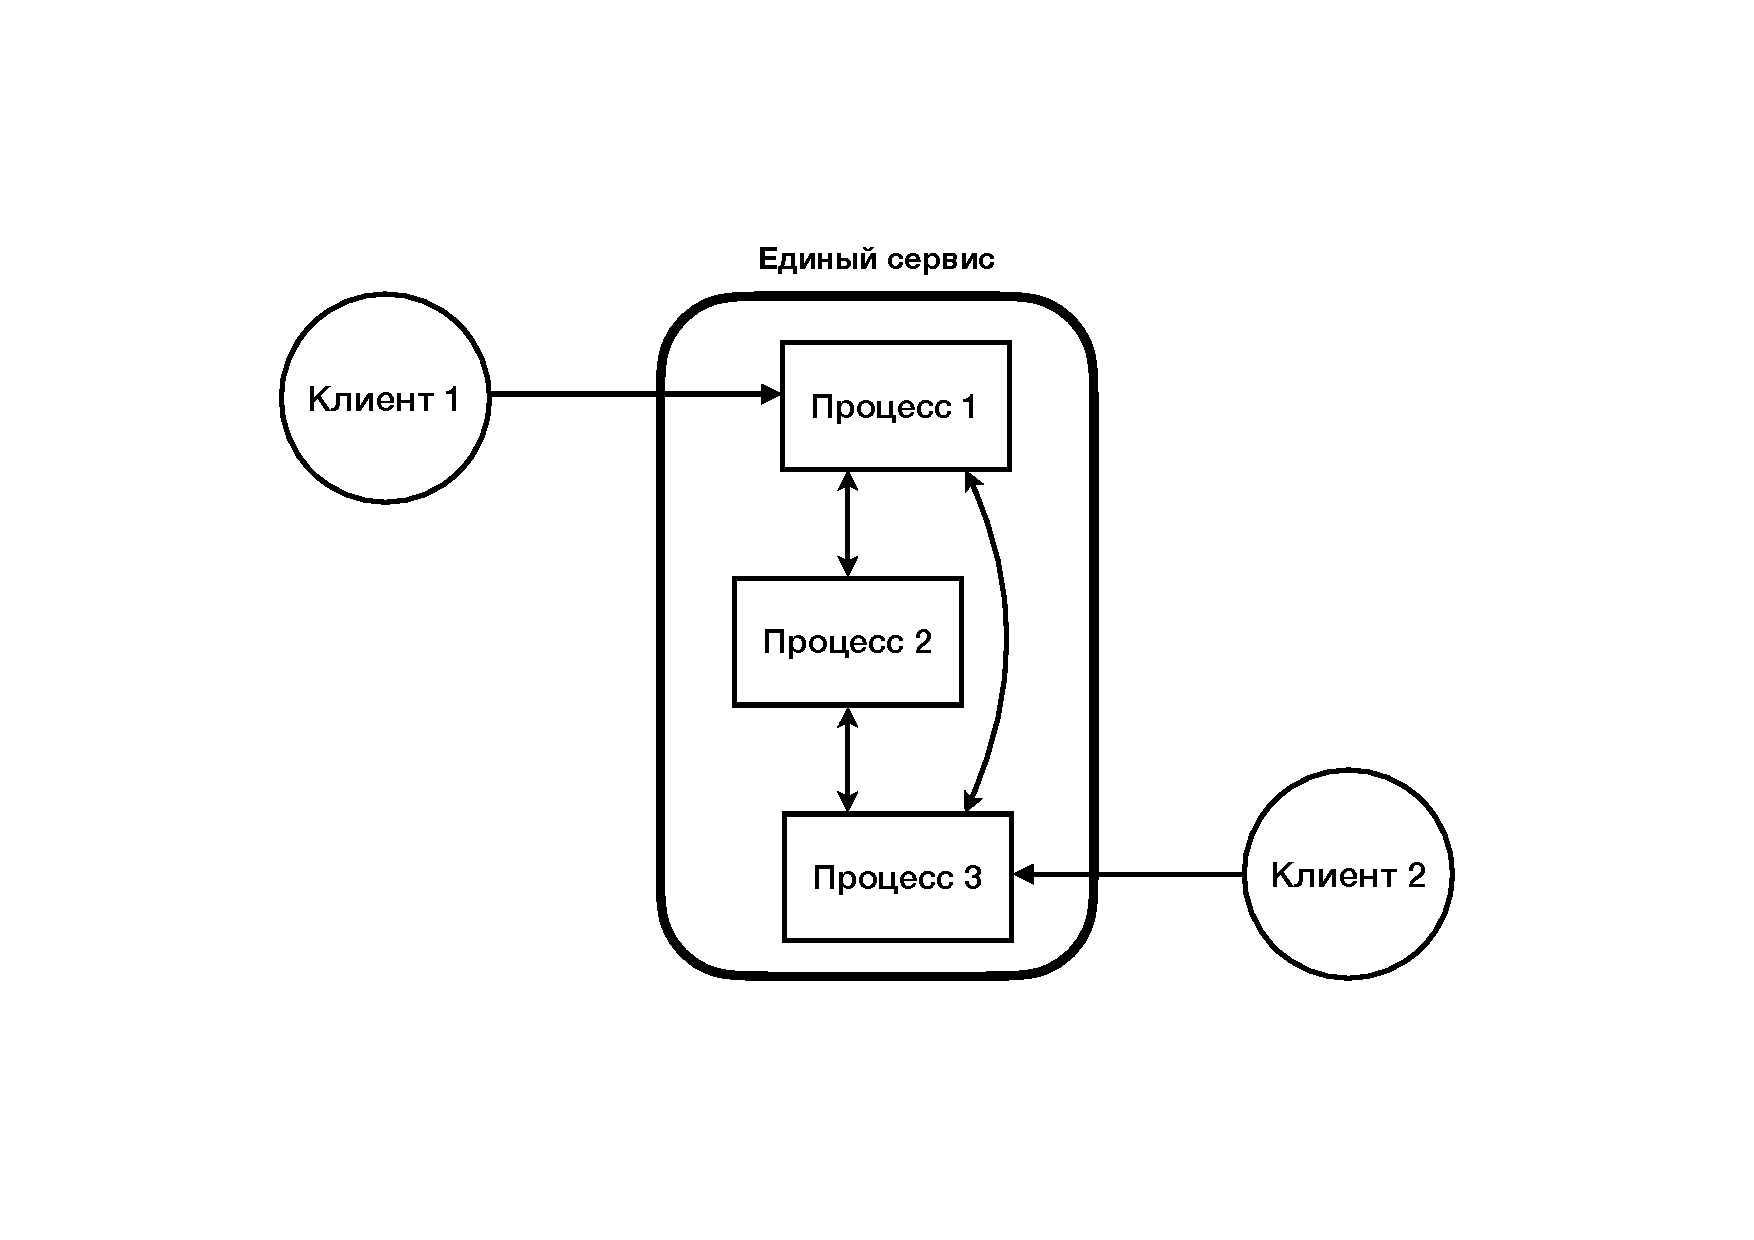
\includegraphics[scale=0.7]{16/MultiSerrver.pdf}
\\
Например на картинке изображён единый сервис с тремя процессами, которые общаются между собой. "Клиент 1"\ обратился в "процесс 1"\, а "клиент 2"\ - в "процесс 3"\, но при этом для них не должна быть заметна какая либо разница в работе с сервисом.

По большому счёту такая система - это клиент-сервер.

\item
Сервера приложений - может быть много серверов и один сервер может быть клиентом другого сервера.
Например подход MVC (Model-View-Controller): \\клиент <--> сервер <--> база данных.

MVC - схема разделения данных приложения и управляющей логики на три отдельных компонента: модель (хранение данных), представление (данных) и контроллер (обработка) — таким образом, что модификация каждого компонента может осуществляться независимо

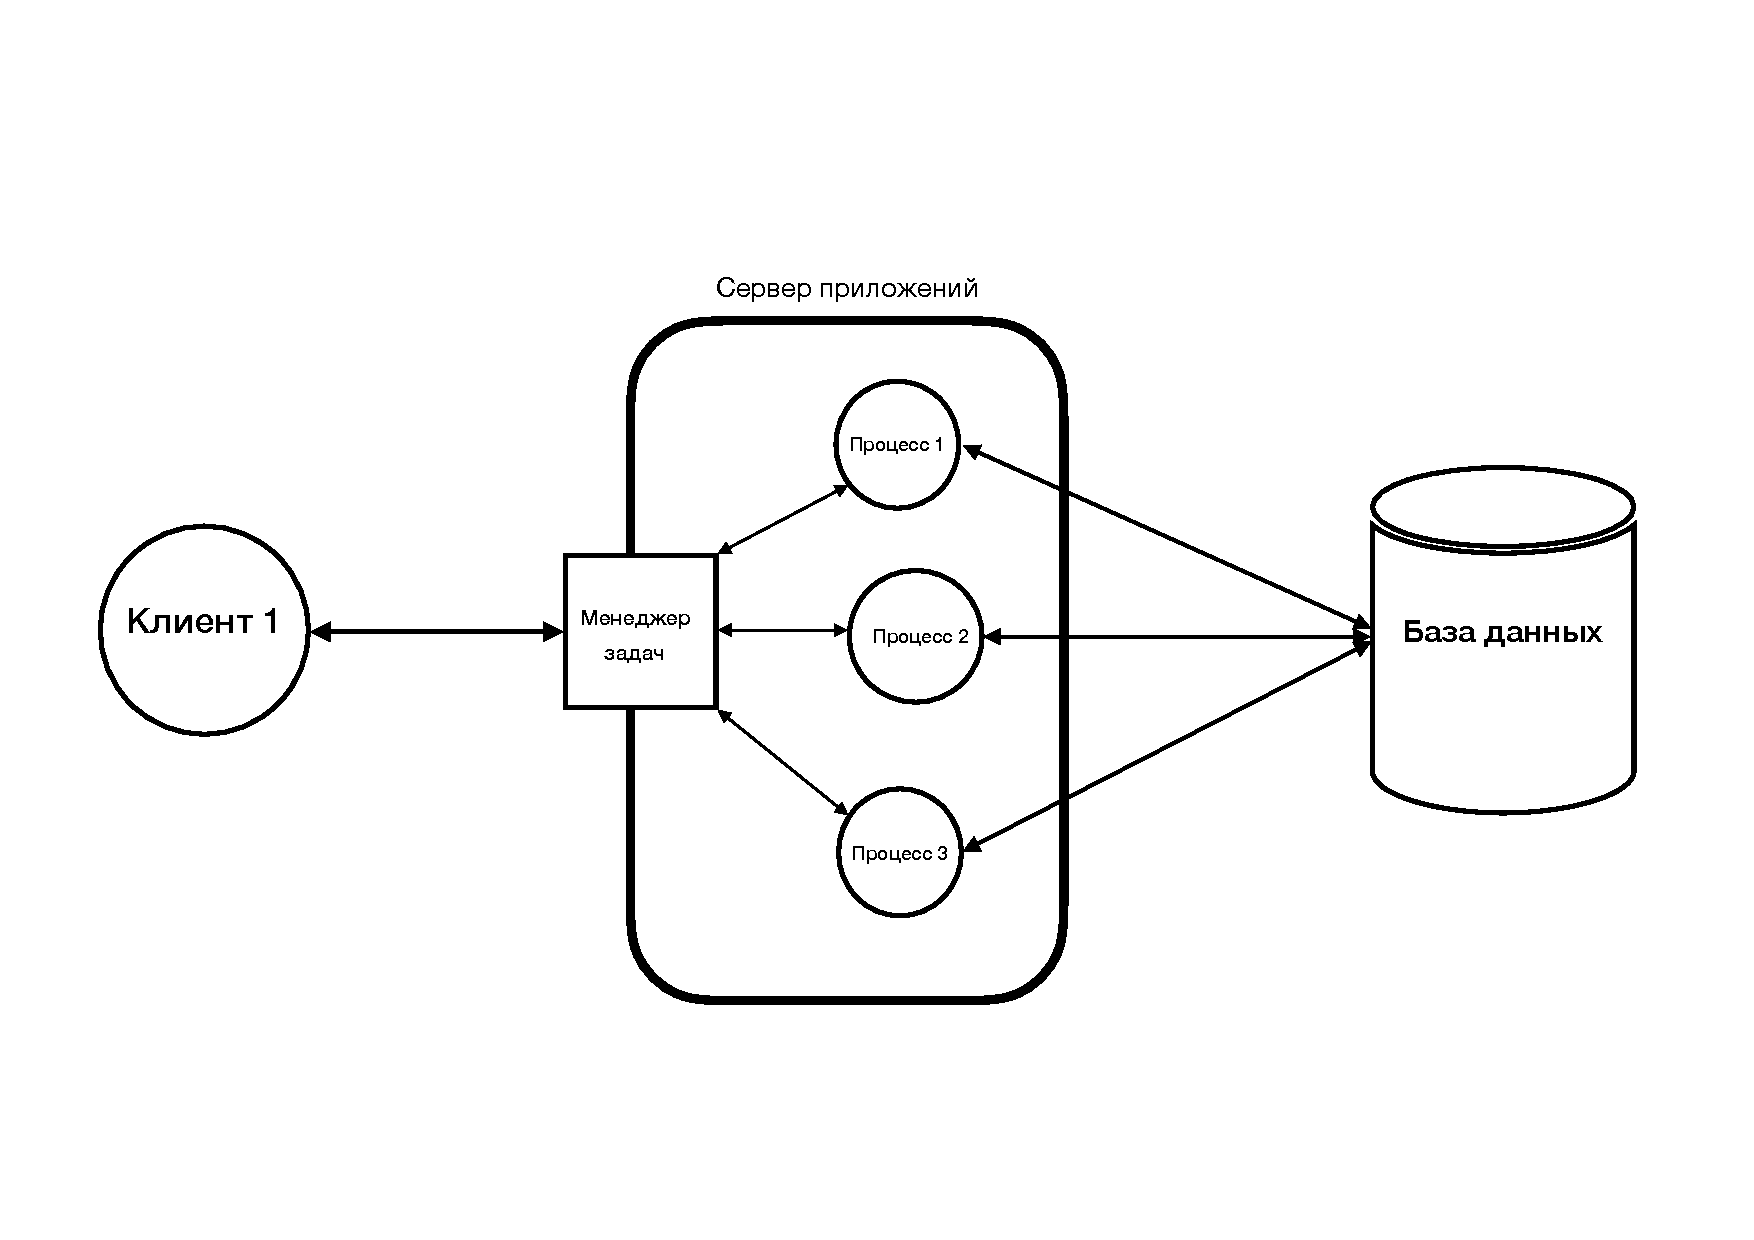
\includegraphics[scale=0.6]{16/Model-View-Controller.pdf}

К примеру система на картинке. В ней модель - база данных, представление данных - клиент, а контроллер - сервер приложений.\\
База данных выполняет только операции с данными (SQL запросы), а сервер приложений выполняет всю бизнес-логику, также может содержать некий объект, который раскидывает задачи на процессы, которые выполняют какие-то задачи и, при необходимости, обращаются к базе данных.
Клиент обычно не делает содержательной работы и отвечает только за ввод данных и отображение результатов (к примеру веб браузер).

\end{itemize}

\item \textbf{ Одноранговая}

Вообще никаких серверов не выделяется, нет ни главного процесса, ни клиента, все участники равноправны (например сеть торрент).

\end{enumerate}



















